\documentclass[10pt,handout]{beamer}\usepackage[]{graphicx}\usepackage[]{color}
% maxwidth is the original width if it is less than linewidth
% otherwise use linewidth (to make sure the graphics do not exceed the margin)
\makeatletter
\def\maxwidth{ %
  \ifdim\Gin@nat@width>\linewidth
    \linewidth
  \else
    \Gin@nat@width
  \fi
}
\makeatother

\definecolor{fgcolor}{rgb}{0.345, 0.345, 0.345}
\newcommand{\hlnum}[1]{\textcolor[rgb]{0.686,0.059,0.569}{#1}}%
\newcommand{\hlstr}[1]{\textcolor[rgb]{0.192,0.494,0.8}{#1}}%
\newcommand{\hlcom}[1]{\textcolor[rgb]{0.678,0.584,0.686}{\textit{#1}}}%
\newcommand{\hlopt}[1]{\textcolor[rgb]{0,0,0}{#1}}%
\newcommand{\hlstd}[1]{\textcolor[rgb]{0.345,0.345,0.345}{#1}}%
\newcommand{\hlkwa}[1]{\textcolor[rgb]{0.161,0.373,0.58}{\textbf{#1}}}%
\newcommand{\hlkwb}[1]{\textcolor[rgb]{0.69,0.353,0.396}{#1}}%
\newcommand{\hlkwc}[1]{\textcolor[rgb]{0.333,0.667,0.333}{#1}}%
\newcommand{\hlkwd}[1]{\textcolor[rgb]{0.737,0.353,0.396}{\textbf{#1}}}%
\let\hlipl\hlkwb

\usepackage{framed}
\makeatletter
\newenvironment{kframe}{%
 \def\at@end@of@kframe{}%
 \ifinner\ifhmode%
  \def\at@end@of@kframe{\end{minipage}}%
  \begin{minipage}{\columnwidth}%
 \fi\fi%
 \def\FrameCommand##1{\hskip\@totalleftmargin \hskip-\fboxsep
 \colorbox{shadecolor}{##1}\hskip-\fboxsep
     % There is no \\@totalrightmargin, so:
     \hskip-\linewidth \hskip-\@totalleftmargin \hskip\columnwidth}%
 \MakeFramed {\advance\hsize-\width
   \@totalleftmargin\z@ \linewidth\hsize
   \@setminipage}}%
 {\par\unskip\endMakeFramed%
 \at@end@of@kframe}
\makeatother

\definecolor{shadecolor}{rgb}{.97, .97, .97}
\definecolor{messagecolor}{rgb}{0, 0, 0}
\definecolor{warningcolor}{rgb}{1, 0, 1}
\definecolor{errorcolor}{rgb}{1, 0, 0}
\newenvironment{knitrout}{}{} % an empty environment to be redefined in TeX

\usepackage{alltt}


%\input{slides_header.tex}
\input{/home/sahir/git_repositories/epib607/inst/slides/slides_header2.tex}
\graphicspath{{/home/sahir/git_repositories/epib607/inst/slides/figure/}}


\newcommand{\Var}{\operatorname{Var}}
\newcommand{\Expec}{\operatorname{E}}
\newcommand{\Prob}{\operatorname{P}}

%\let\oldShaded\Shaded
%\let\endoldShaded\endShaded
%\renewenvironment{Shaded}{\footnotesize\oldShaded}{\endoldShaded}

%\newcommand{\blue}[1]{\textcolor{blue}{#1}}
%\newcommand{\red}[1]{\textcolor{red}{#1}}


\usepackage{xparse}
\NewDocumentCommand\mylist{>{\SplitList{;}}m}
{
	\begin{itemize}
		\ProcessList{#1}{ \insertitem }
	\end{itemize}
}
\NewDocumentCommand\mynum{>{\SplitList{;}}m}
{
	\begin{enumerate}
		\ProcessList{#1}{ \insertitem }
	\end{enumerate}
}
\newcommand\insertitem[1]{\item #1}

\newcommand\FrameText[1]{%
	\begin{textblock*}{\paperwidth}(0pt,\textheight)
		\raggedright #1\hspace{.5em}
\end{textblock*}}
\IfFileExists{upquote.sty}{\usepackage{upquote}}{}
\begin{document}
	
	
	


	\title{021 - Introduction to Regression}
\author{EPIB 607}
\institute{
	Sahir Rai Bhatnagar\\
	Department of Epidemiology, Biostatistics, and Occupational Health\\
	McGill University\\
	
	\vspace{0.1 in}
	
	\texttt{sahir.bhatnagar@mcgill.ca}\\
	%\texttt{\url{https://sahirbhatnagar.com/EPIB607/}}
}

\date{slides compiled on \today}

\maketitle


\section{Parameter-contrasts}

\begin{frame}{Introduction to parameter-contrasts}
	
	\begin{itemize}
		\setlength\itemsep{2em}
		\item We started the course by talking about the case where there were no determinants, i.e., no subpopulations $\to$ there was one global parameter ($\mu$, $\pi$, $\lambda$). \pause 
		\item Now we concern ourselves with determinants of the global parameter. For example:
		\begin{itemize}
			\item $\mu_{north}$ vs. $\mu_{south}$
			\item $\pi_{north}$ vs. $\pi_{south}$
			\item $\lambda_{north}$ vs. $\lambda_{south}$
		\end{itemize}
		
		\item Today we introduce population parameter \underline{contrasts} in a regression framework
		
	\end{itemize}
	
\end{frame}


\begin{frame}{Why regression for parameter-contrasts?}
	
	\begin{itemize}
		\setlength\itemsep{1.5em}
		\item Why do we start in a regression framework (as opposed to two-sample inference in DVB)?  
		\item \textbf{Parameter contrasts are a special case of regression}  
	%	\item Approach taken in Miettinen, Clayton in Hills, Rothman and Greenland, baby Rothman
	\end{itemize}
	
\end{frame}


\begin{frame}{What is regression?}
	
	\begin{itemize}
		\setlength\itemsep{2em}
		\item How \textbf{parameters} relate to its determinants 
		\item How to link the parameters between the different populations through generic equations, that looks like a regression equation.  
		\item Then once you get data, you can actually fit or get your best estimates of those parameters
	\end{itemize}
	
\end{frame}

\begin{frame}{Linear regression: The Concept}
	
	\begin{itemize}
		\setlength\itemsep{2em}
		\item A regression model is said to be \textbf{linear} when it is of the form 
		\begin{align*}
			\mu & = \mu_0 + \sum_{j=1}^p \beta_j X_j \\
			& = \mu_0 + \beta_1 X_1 +  \beta_1 X_1 + \cdots +  \beta_p X_p
		\end{align*}
		
		\item Which means that the value of the mean ($\mu$) is viewed as a linear combination of the parameters $\mu_0, \beta_1, \beta_2, \ldots, \beta_p$, the coefficients of the linear combination being the realizations for the $X$'s
		
	\end{itemize}
	
\end{frame}

\begin{frame}{Linear regression: Example}
	
	\begin{itemize}
		\setlength\itemsep{2em}
		\item Consider the depths of the ocean example
		\item Here, $\mu$ designates the true mean depth of the ocean 
		\item For this parameter, one might consider the determinant 
		\begin{itemize}
			\item $X$ which is an indicator variable defined by			
			$$
			X = \begin{cases}
			1 & \textrm{if Southern hemisphere}\\
			0 & \textrm{if Northern hemisphere}
			\end{cases}
			$$
			
		\end{itemize} 
		
	\end{itemize}
	
\end{frame}



\begin{frame}{Linear regression: Example}
	
	\begin{itemize}
		\setlength\itemsep{1.7em}
		\item The model might be taken as 
		$$
		\mu_X = \mu_0 + \beta_1 \cdot X 
		$$
		
		and provides the mean depth of the ocean \underline{given} $X$ 
		
		\item The subscript $X$ indicates that $\mu$ depends on the value of $x$
		
		\item The mean depth of the ocean $\mu_X$ is a linear combination of $\mu_0$ and $\beta_1$ 
		
			
		\item If we had an infinite amount of data, the mean depth of the ocean would be determined by hemisphere:
		
		$$
		\mu_X = \begin{cases}
		\mu_0 + \beta_1  &  \textrm{if Southern hemisphere}\\
		\mu_0  &  \textrm{if Northern Hemisphere}
		\end{cases}
		$$
		
	\end{itemize}
	
\end{frame}



\begin{comment}
\section{Regression equations when the truth is known}


\begin{frame}{Don't we need a cloud of points to have a regression line?}
	\pause 
	\begin{itemize}
		\item Although many courses and textbooks introduce regression concepts this way, the answer is \textbf{NO}. \pause 
		
		\item There is nothing in the regression formulation that specifies at which 'X' values the mean Y values at these X values are to be determined. Unlike many textbboks that start with Xs on a 'continuous' scale, and then later have to deal with a 2-point (binary) X, we are starting with this simplest case, and will move 'up' later. 
		
		\item We are doing this for a few reasons: in epidemiology, the first and simplest contrasts involve just two categories, the reference category and the index category; a simple subtraction of 2 parameter values is easier to do and to explain to a lay person; and there is no argument about how the function behaves at the values between 0 and 1:  There are no parameter values at Male = 0.4 or Male = 1.4, they are only at Male=0 and Male=1. 
 
	\end{itemize}
\end{frame}

\begin{frame}{Don't we need a cloud of points to have a regression line?}
	
		\begin{itemize}
			
		\item In addition, it is easier to learn the fundamental concepts and principles of regression if we can easily 'see' what exactly is going on. Fewer blackbox formulae mean more transparency and understanding. \pause 
		
		\item As we will see later on, when we have a value for a dental health parameter (eg the mean number of decayed, missing and filled DMF teeth) at X = 0 parts per million of fluoride in the drinking water, and another parameter value at X = 1 parts per million, we can only look at these 2 parameter values. If this is not enough, we would need to have (obtain) parameter values at the intermediate fluoride levels, or levels beyond 1 ppm, to trace out the full parameter relation, namely  how the mean-DMF varies as a function of fluoride levels. If we have large numbers of observations at each level, then the DMF means will trace out a smooth curve. If data are limited, and the trace is jumpy/wobbly, we will probably resort to a sensible smooth function, the coefficients of which will have to be estimated from (fitted to) data. 
	\end{itemize}
\end{frame}




\begin{frame}{Relative differences (ratios) expressed in numbers}
	
	\begin{itemize}
		\item A ratio can be more helpful than a difference, especially if you are don't have a sense of how large the parameter value is even in the reference category. As an example, on average, how many more red blood cells do men have than women? or how much faster  are gamers' reaction times compared with nongamers? \pause 
		\item Recall our hypothetical mean ocean depths, 3.6 Km  in the oceans in the Northern hemisphere (reference category) and 4.5Km in the oceans of the Southern hemisphere (index category). Thus, the S:N (South divided by North) ratio is 4.5/3.6 or 1.25.
	\end{itemize}
\end{frame}	
	
	
	\begin{frame}[fragile,plain]
\begin{knitrout}\tiny
\definecolor{shadecolor}{rgb}{0.969, 0.969, 0.969}\color{fgcolor}

{\centering 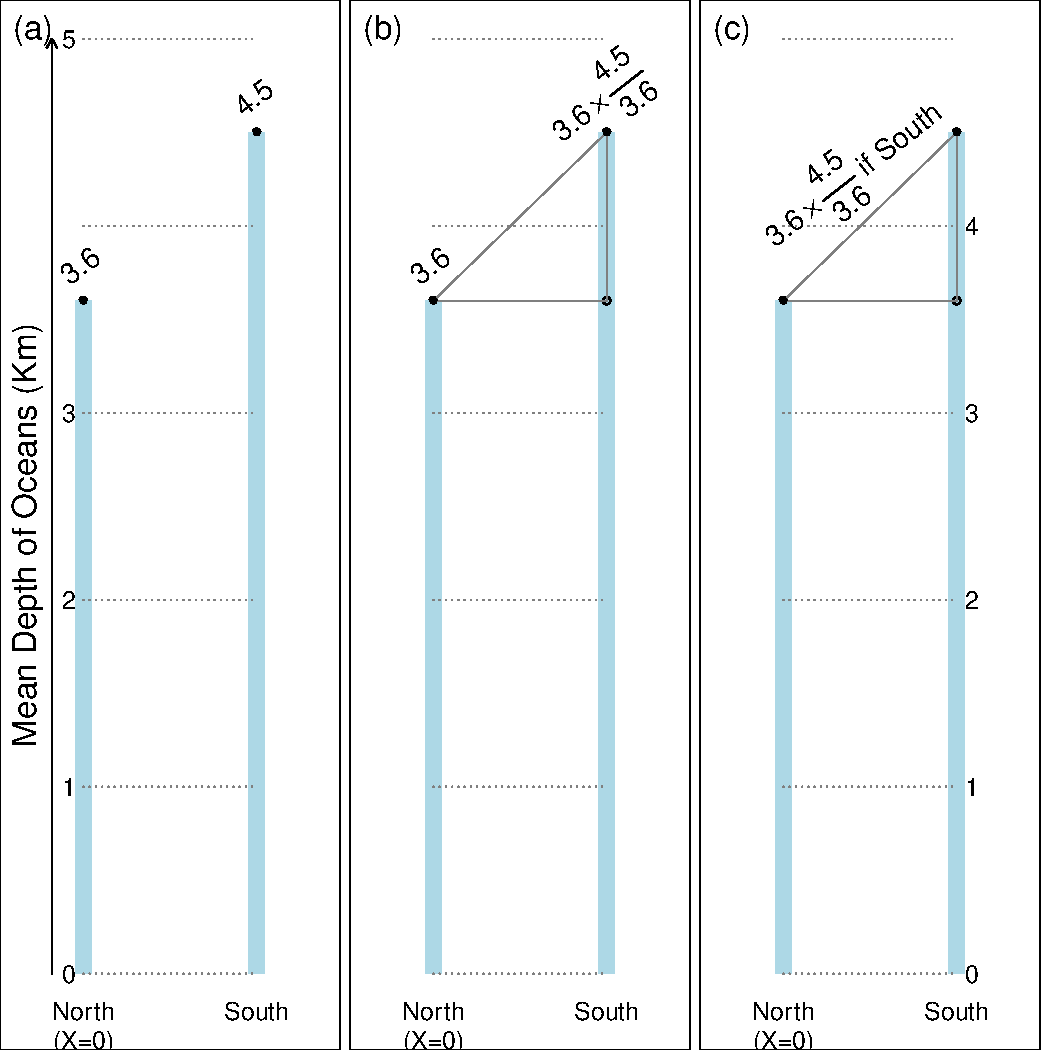
\includegraphics[width=0.7\textwidth]{figure/unnamed-chunk-2-1} 

}


\end{knitrout}
	\end{frame}
	

	\begin{frame}[fragile]{Relative differences (ratios) -- expressed in symbols}
			
		\begin{itemize}
			\item To rewrite these numbers in a symbolic equation suitable for a computer, we  again convert the logical `if South` to a numerical Southern-hemisphere-indicator, using the binary variate $X$ that takes the value 0 if the Northern hemisphere, and  1 if the Southern hemisphere.
			
			\item But go back to  some long-forgotten mathematics from high school to be able to tell the computer to toggle the ratio off and on. Recall \textbf{powers} of numbers, where, for example, 
			`$y$ to the power 2', or $y^2$ is the square of $y$. 
			
			\item The two powers we exploit are 0 and 1. `$y$ to the power 1', or $y^1$ is just $y$ and `$y$ to the power 0', or $y^0$ is 1.
			

		\end{itemize}
			
			
	\end{frame}
	
	
		\begin{frame}[fragile]{Relative differences (ratios) -- expressed in symbols}
		
		\begin{itemize}
	
			
			\item We take advantage of these to write
			$$\mu_X = \mu \ | \ X  \ = \mu_0 \ \times \  \Big\{ \frac{\mu_{South}}{\mu_{North}}\Big\}^X = \mu_0 \ \times Ratio \ ^ X.$$ 
			
			\item You can check that it works for each hemisphere by setting $X=0$ and $X=1$ in turn.
			
			\item Thus, $$\log(y^X) = X \times \log(y)$$  
		\end{itemize}
		
		
	\end{frame}
	
	
	
	

	
	\begin{frame}[fragile,plain]
	
\begin{knitrout}\tiny
\definecolor{shadecolor}{rgb}{0.969, 0.969, 0.969}\color{fgcolor}

{\centering 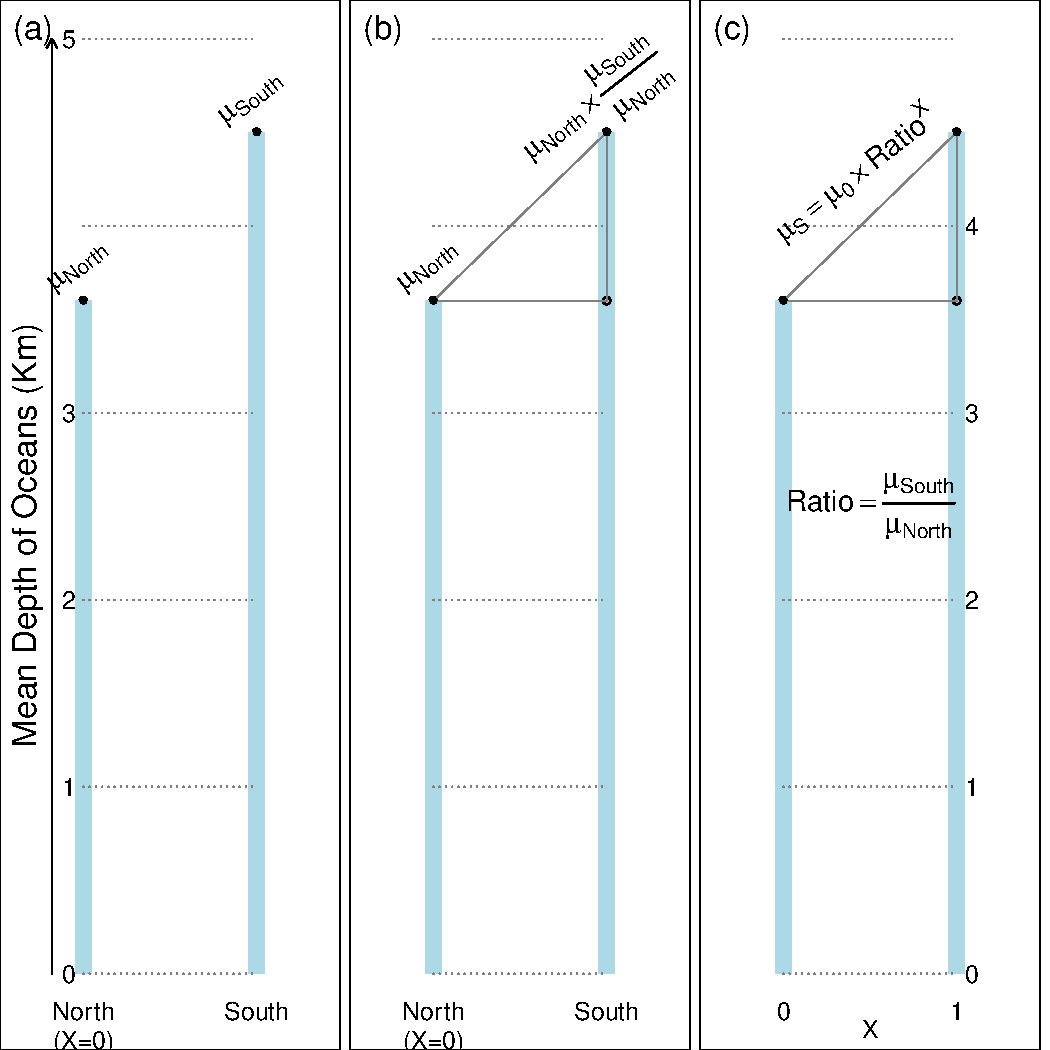
\includegraphics[width=0.7\textwidth]{figure/unnamed-chunk-3-1} 

}


\end{knitrout}
	
\end{frame}
	
	
	
		\begin{frame}[fragile]{Relative differences (ratios) -- expressed in symbols}
		
		\begin{itemize}
			\item Although this is a compact and direct way to express the parameter relation, it is not well suited for fitting these equations to data. 
	
	\item However, in those same  high school mathematics courses, you also learned about \textbf{logarithms}. For example, that 
	$$\log(A \times B) = \log(A) + \log(B); \ \  \log(y^x) = x \times \log(y).$$
	
	\item Thus, we can rewrite the equation in panel (c) as
	
	$$\log(\mu_X) = \log(\mu \ | \ X)  \ = \underbrace{\log(\mu_0)} \ +  \underbrace{\log(Ratio)} \times \ X.$$
	
	\item This has the same 'linear in the two parameters' form as the one for the parameter difference: the parameters are
	$\underbrace{\log(\mu_0)}$ and $\underbrace{\log(Ratio)}$ and they are made into the following 'linear compound' or 'linear predictor':
	$$\log(\mu_X) = \log(\mu \ | \ X)  \ = \underbrace{\log(\mu_0)} \times \ 1 \ + \underbrace{\log(Ratio)} \times \ X.$$
	
	\item The course is concerned with using \textit{regression} software to  \textit{fit/estimate} these 2 parameters from $n$ depth measurements indexed by $X$.

\end{itemize}
	
\end{frame}


\begin{frame}
	\Wider[8em]{
		\centering
		\includegraphics[width=4.9in,height=3.6in]{Fig11.pdf}
	}
\end{frame}


\begin{frame}
	\Wider[8em]{
		\centering
		\includegraphics[width=4.9in,height=3.6in]{Fig12.pdf}
	}
\end{frame}

\begin{frame}
	\Wider[8em]{
		\centering
		\includegraphics[width=4.9in,height=3.6in]{Fig13.pdf}
	}
\end{frame}


\begin{frame}
	\Wider[8em]{
		\centering
		\includegraphics[width=4.9in,height=3.6in]{Fig14.pdf}
	}
\end{frame}


\begin{frame}
	\Wider[8em]{
		\centering
		\includegraphics[width=4.9in,height=3.6in]{Fig15.pdf}
	}
\end{frame}


\begin{frame}
	\Wider[8em]{
		\centering
		\includegraphics[width=4.9in,height=3.6in]{Fig16.pdf}
	}
\end{frame}
\end{comment}

\section{Fitting the regression equation with our sample data}



\begin{frame}[fragile]{Depths of the ocean: North vs. South Hemisphere}
	
\begin{knitrout}\tiny
\definecolor{shadecolor}{rgb}{0.969, 0.969, 0.969}\color{fgcolor}\begin{kframe}
\begin{alltt}
\hlcom{# load function to get depths}
\hlkwd{source}\hlstd{(}\hlstr{"https://raw.githubusercontent.com/sahirbhatnagar/EPIB607/master/inst/labs/
        003-ocean-depths/automate_water_task.R"}\hlstd{)}

\hlcom{# get 1000 depths}
\hlkwd{set.seed}\hlstd{(}\hlnum{222333444}\hlstd{)}
\hlstd{depths} \hlkwb{<-} \hlkwd{automate_water_task}\hlstd{(}\hlkwc{index} \hlstd{=} \hlkwd{sample}\hlstd{(}\hlnum{1}\hlopt{:}\hlnum{50000}\hlstd{,} \hlnum{1000}\hlstd{),}
\hlkwc{student_id} \hlstd{=} \hlnum{222333444}\hlstd{,} \hlkwc{type} \hlstd{=} \hlstr{"depth"}\hlstd{)}

\hlcom{# separate by north and south hemisphere}
\hlstd{depths_north} \hlkwb{<-} \hlstd{depths[}\hlkwd{which}\hlstd{(depths}\hlopt{$}\hlstd{lat}\hlopt{>}\hlnum{0}\hlstd{),]}
\hlstd{depths_south} \hlkwb{<-} \hlstd{depths[}\hlkwd{which}\hlstd{(depths}\hlopt{$}\hlstd{lat}\hlopt{<}\hlnum{0}\hlstd{),]}

\hlcom{# restrict sample to 200 (at random)}
\hlstd{depths_north} \hlkwb{<-} \hlstd{depths_north[}\hlkwd{sample}\hlstd{(}\hlnum{1}\hlopt{:}\hlkwd{nrow}\hlstd{(depths_north),} \hlnum{200}\hlstd{), ]}
\hlstd{depths_south} \hlkwb{<-} \hlstd{depths_south[}\hlkwd{sample}\hlstd{(}\hlnum{1}\hlopt{:}\hlkwd{nrow}\hlstd{(depths_south),} \hlnum{200}\hlstd{), ]}

\hlcom{# add indicator variable}
\hlstd{depths_north}\hlopt{$}\hlstd{South} \hlkwb{<-} \hlnum{0}
\hlstd{depths_south}\hlopt{$}\hlstd{South} \hlkwb{<-} \hlnum{1}

\hlcom{# combine data}
\hlstd{depths} \hlkwb{<-} \hlkwd{rbind}\hlstd{(depths_north, depths_south)}
\hlkwd{head}\hlstd{(depths)}

\hlcom{# calculate mean and sd by hemisphere}
    \hlstd{mean.sd} \hlkwb{<-} \hlstd{depths} \hlopt \hlkwd{group_by}\hlstd{(South)} \hlopt
    \hlkwd{summarise}\hlstd{(}\hlkwc{means} \hlstd{=} \hlkwd{mean}\hlstd{(alt),} \hlkwc{sds} \hlstd{=} \hlkwd{sd}\hlstd{(alt))}

    \hlstd{means} \hlkwb{<-} \hlstd{mean.sd}\hlopt{$}\hlstd{means}
    \hlstd{sds} \hlkwb{<-} \hlstd{mean.sd}\hlopt{$}\hlstd{sds}
\end{alltt}
\end{kframe}
\end{knitrout}
	
	
\end{frame}


\begin{frame}[fragile]{Depths of the ocean: North vs. South Hemisphere}
	
\begin{knitrout}\tiny
\definecolor{shadecolor}{rgb}{0.969, 0.969, 0.969}\color{fgcolor}

{\centering 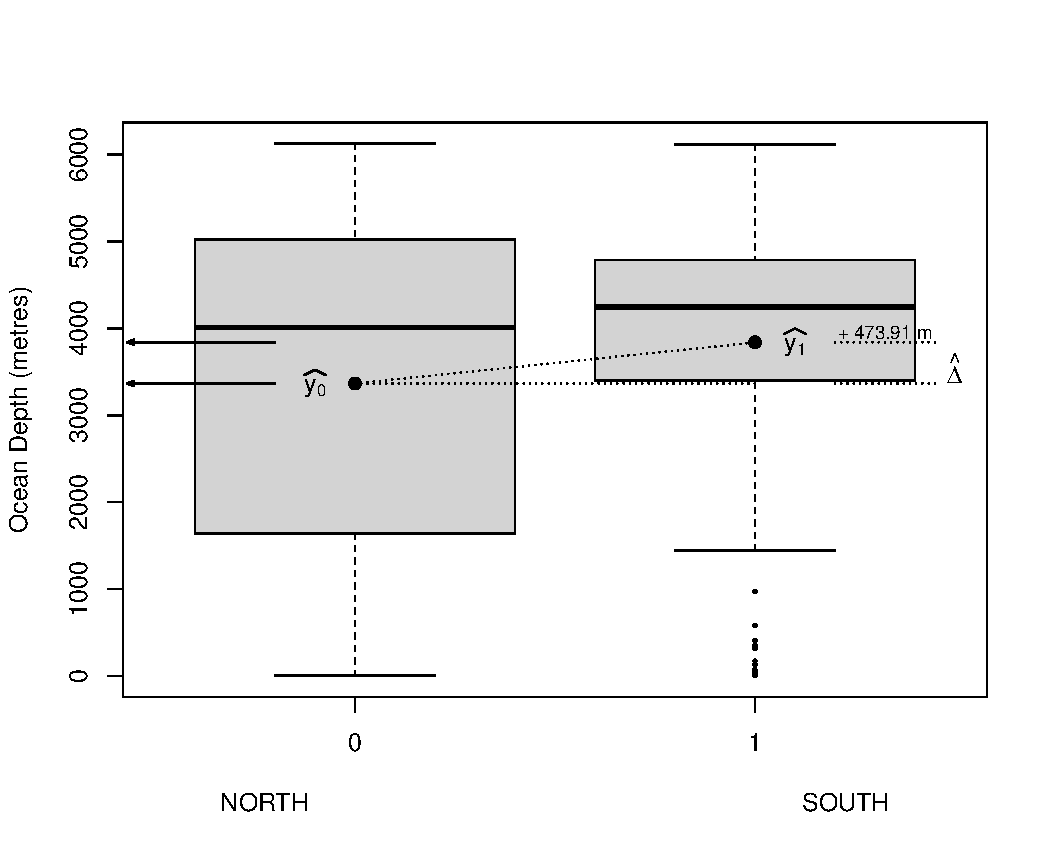
\includegraphics[width=\maxwidth]{figure/unnamed-chunk-5-1} 

}


\end{knitrout}
	
	
\end{frame}



\begin{frame}[fragile]{Standard error of the mean difference}
	
	To perform inference we first need to calculate the SE of the mean difference given by:
	
	\begin{equation}
		SE_{\bar{y_1} - \bar{y_0}} = \sqrt{\frac{s_0^2}{n_0} + \frac{s_1^2}{n_1}}
	\end{equation}
	
	\pause 
	
\begin{knitrout}\scriptsize
\definecolor{shadecolor}{rgb}{0.969, 0.969, 0.969}\color{fgcolor}\begin{kframe}
\begin{alltt}
\hlstd{n0} \hlkwb{<-} \hlkwd{nrow}\hlstd{(depths_north)}
\hlstd{n1} \hlkwb{<-} \hlkwd{nrow}\hlstd{(depths_south)}

\hlstd{mean0} \hlkwb{<-} \hlkwd{mean}\hlstd{(depths_north}\hlopt{$}\hlstd{alt)}
\hlstd{mean1} \hlkwb{<-} \hlkwd{mean}\hlstd{(depths_south}\hlopt{$}\hlstd{alt)}

\hlstd{var0} \hlkwb{<-} \hlkwd{var}\hlstd{(depths_north}\hlopt{$}\hlstd{alt)}
\hlstd{var1} \hlkwb{<-} \hlkwd{var}\hlstd{(depths_south}\hlopt{$}\hlstd{alt)}

\hlstd{(SEM} \hlkwb{<-} \hlkwd{sqrt}\hlstd{(var0}\hlopt{/}\hlstd{n0} \hlopt{+} \hlstd{var1}\hlopt{/}\hlstd{n1))}
\end{alltt}
\begin{verbatim}
## [1] 171.4861
\end{verbatim}
\end{kframe}
\end{knitrout}
	
	
\end{frame}



\begin{frame}[fragile]{95\% Confidence Interval for the Mean Difference}
	
	We can then calculate a 95\% CI for the mean difference given by:
	
	\begin{equation}
		(\bar{y_1} - \bar{y_0}) \pm t^\star_{(n_0 + n_1 - 2)} \times SE_{\bar{y_1} - \bar{y_0}}
	\end{equation}
	
	\pause 
	
\begin{knitrout}\scriptsize
\definecolor{shadecolor}{rgb}{0.969, 0.969, 0.969}\color{fgcolor}\begin{kframe}
\begin{alltt}
\hlcom{# assuming equal variances}
\hlstd{(mean1} \hlopt{-} \hlstd{mean0)} \hlopt{+} \hlkwd{qt}\hlstd{(}\hlkwd{c}\hlstd{(}\hlnum{0.025}\hlstd{,} \hlnum{0.975}\hlstd{),} \hlkwc{df} \hlstd{= n0} \hlopt{+} \hlstd{n1} \hlopt{-} \hlnum{2}\hlstd{)} \hlopt{*} \hlstd{SEM}
\end{alltt}
\begin{verbatim}
## [1] 136.7782 811.0418
\end{verbatim}
\begin{alltt}
\hlcom{# similar to z interval}
\hlkwd{qnorm}\hlstd{(}\hlkwd{c}\hlstd{(}\hlnum{0.025}\hlstd{,} \hlnum{0.975}\hlstd{),} \hlkwc{mean} \hlstd{= mean1} \hlopt{-} \hlstd{mean0,} \hlkwc{sd} \hlstd{= SEM)}
\end{alltt}
\begin{verbatim}
## [1] 137.8034 810.0166
\end{verbatim}
\end{kframe}
\end{knitrout}
	
	
\end{frame}


\begin{frame}[fragile]{Parameter contrasts with regression}
	
	Using the \texttt{lm} function in \texttt{R}:
	
	
\begin{knitrout}\scriptsize
\definecolor{shadecolor}{rgb}{0.969, 0.969, 0.969}\color{fgcolor}\begin{kframe}
\begin{alltt}
\hlcom{# regression. lm assumes equal variances}
\hlstd{fit} \hlkwb{<-} \hlkwd{lm}\hlstd{(alt} \hlopt{~} \hlstd{South,} \hlkwc{data} \hlstd{= depths)}
\hlkwd{summary}\hlstd{(fit)}
\end{alltt}
\begin{verbatim}
## Coefficients:
##             Estimate Std. Error t value Pr(>|t|)    
## (Intercept)   3365.6      121.3  27.755  < 2e-16 ***
## South          473.9      171.5   2.764  0.00598 ** 
## ---
## Signif. codes:  0 '***' 0.001 '**' 0.01 '*' 0.05 '.' 0.1 ' ' 1
## 
## Residual standard error: 1715 on 398 degrees of freedom
## Multiple R-squared: 0.01883,	Adjusted R-squared: 0.01636 
## F-statistic: 7.637 on 1 and 398 DF,  p-value: 0.005983
\end{verbatim}
\end{kframe}
\end{knitrout}
	
	
\end{frame}


\begin{frame}[fragile]{Confidence interval from regression fit}
	
\begin{knitrout}\scriptsize
\definecolor{shadecolor}{rgb}{0.969, 0.969, 0.969}\color{fgcolor}\begin{kframe}
\begin{alltt}
\hlkwd{confint}\hlstd{(fit)}
\end{alltt}
\begin{verbatim}
##                 2.5 %    97.5 %
## (Intercept) 3127.2068 3603.9832
## South        136.7782  811.0418
\end{verbatim}
\end{kframe}
\end{knitrout}
	
	
\end{frame}



\begin{frame}[fragile]{Unequal variances using \texttt{stats::t.test}}
	
	\texttt{stats::t.test} assumes unequal variances by default:
	
	
\begin{knitrout}\scriptsize
\definecolor{shadecolor}{rgb}{0.969, 0.969, 0.969}\color{fgcolor}\begin{kframe}
\begin{alltt}
\hlstd{stats}\hlopt{::}\hlkwd{t.test}\hlstd{(alt} \hlopt{~} \hlstd{South,} \hlkwc{data} \hlstd{= depths,} \hlkwc{var.equal} \hlstd{=} \hlnum{FALSE}\hlstd{)}
\end{alltt}
\begin{verbatim}
## Welch Two Sample t-test with alt by South 
## t = -2.7635, df = 356.262, p-value = 0.006015
## alternative hypothesis: true difference in means between group 0 and group 1 is not equal to 0 
## 95 percent confidence interval:
##  -811.1623 -136.6577 
## sample estimates:
## mean in group 0 mean in group 1 
##        3365.595        3839.505
\end{verbatim}
\begin{alltt}
\hlstd{(mean0} \hlopt{-} \hlstd{mean1)} \hlopt{+} \hlkwd{qt}\hlstd{(}\hlkwd{c}\hlstd{(}\hlnum{0.025}\hlstd{,} \hlnum{0.975}\hlstd{),} \hlkwc{df} \hlstd{=} \hlnum{349.61783}\hlstd{)} \hlopt{*} \hlstd{SEM}
\end{alltt}
\begin{verbatim}
## [1] -811.1841 -136.6359
\end{verbatim}
\end{kframe}
\end{knitrout}
	
	
\end{frame}



\begin{frame}[fragile]{Equal variances using \texttt{stats::t.test}}
	
	We can specify equal variance assumption in \texttt{stats::t.test}:
	
\begin{knitrout}\scriptsize
\definecolor{shadecolor}{rgb}{0.969, 0.969, 0.969}\color{fgcolor}\begin{kframe}
\begin{alltt}
\hlstd{stats}\hlopt{::}\hlkwd{t.test}\hlstd{(alt} \hlopt{~} \hlstd{South,} \hlkwc{data} \hlstd{= depths,} \hlkwc{var.equal} \hlstd{=} \hlnum{TRUE}\hlstd{)}
\end{alltt}
\begin{verbatim}
##  Two Sample t-test with alt by South 
## t = -2.7635, df = 398, p-value = 0.005983
## alternative hypothesis: true difference in means between group 0 and group 1 is not equal to 0 
## 95 percent confidence interval:
##  -811.0418 -136.7782 
## sample estimates:
## mean in group 0 mean in group 1 
##        3365.595        3839.505
\end{verbatim}
\begin{alltt}
\hlstd{(mean0} \hlopt{-} \hlstd{mean1)} \hlopt{+} \hlkwd{qt}\hlstd{(}\hlkwd{c}\hlstd{(}\hlnum{0.025}\hlstd{,} \hlnum{0.975}\hlstd{),} \hlkwc{df} \hlstd{= n0} \hlopt{+} \hlstd{n1} \hlopt{-} \hlnum{2}\hlstd{)} \hlopt{*} \hlstd{SEM}
\end{alltt}
\begin{verbatim}
## [1] -811.0418 -136.7782
\end{verbatim}
\end{kframe}
\end{knitrout}
	
	
\end{frame}




%\begin{frame}[allowframebreaks]
%\nocite{breiman1984classification}
%	\nocite{friedman2001elements}
%	\nocite{james2013introduction}
%	\nocite{lopez2015arbres}
%	\frametitle{References}
%\printbibliography
%\end{frame}


\begin{frame}[fragile]{Session Info}
	\tiny
	
\begin{knitrout}\tiny
\definecolor{shadecolor}{rgb}{0.969, 0.969, 0.969}\color{fgcolor}\begin{kframe}
\begin{verbatim}
R version 4.1.1 (2021-08-10)
Platform: x86_64-pc-linux-gnu (64-bit)
Running under: Pop!_OS 21.04

Matrix products: default
BLAS:   /usr/lib/x86_64-linux-gnu/openblas-pthread/libblas.so.3
LAPACK: /usr/lib/x86_64-linux-gnu/openblas-pthread/libopenblasp-r0.3.13.so

attached base packages:
[1] tools     stats     graphics  grDevices utils     datasets  methods  
[8] base     

other attached packages:
 [1] DT_0.16           mosaic_1.7.0      Matrix_1.3-2      mosaicData_0.20.1
 [5] ggformula_0.9.4   ggstance_0.3.4    lattice_0.20-41   kableExtra_1.2.1 
 [9] socviz_1.2        gapminder_0.3.0   here_0.1          NCStats_0.4.7    
[13] FSA_0.8.30        forcats_0.5.1     stringr_1.4.0     dplyr_1.0.7      
[17] purrr_0.3.4       readr_1.4.0       tidyr_1.1.4       tibble_3.1.5     
[21] ggplot2_3.3.5     tidyverse_1.3.0   knitr_1.36       

loaded via a namespace (and not attached):
 [1] fs_1.5.0           lubridate_1.7.9    webshot_0.5.2      httr_1.4.2        
 [5] rprojroot_2.0.2    backports_1.2.1    utf8_1.2.2         R6_2.5.1          
 [9] DBI_1.1.1          colorspace_2.0-2   withr_2.4.2        tidyselect_1.1.1  
[13] gridExtra_2.3      leaflet_2.0.3      curl_4.3.2         compiler_4.1.1    
[17] cli_3.0.1          rvest_1.0.0        pacman_0.5.1       xml2_1.3.2        
[21] ggdendro_0.1.22    mosaicCore_0.8.0   scales_1.1.1       digest_0.6.28     
[25] foreign_0.8-81     rmarkdown_2.11.3   rio_0.5.16         pkgconfig_2.0.3   
[29] htmltools_0.5.2    highr_0.9          dbplyr_1.4.4       fastmap_1.1.0     
[33] htmlwidgets_1.5.3  rlang_0.4.12       readxl_1.3.1       rstudioapi_0.13   
[37] farver_2.1.0       generics_0.1.0     jsonlite_1.7.2     crosstalk_1.1.1   
[41] zip_2.2.0          car_3.0-9          magrittr_2.0.1     Rcpp_1.0.7        
[45] munsell_0.5.0      fansi_0.5.0        abind_1.4-5        lifecycle_1.0.1   
[49] stringi_1.7.5      carData_3.0-4      MASS_7.3-53.1      plyr_1.8.6        
[53] grid_4.1.1         blob_1.2.1         ggrepel_0.8.2      crayon_1.4.1      
[57] cowplot_1.1.0      haven_2.3.1        splines_4.1.1      hms_1.1.1         
[61] pillar_1.6.4       reprex_0.3.0       glue_1.4.2         evaluate_0.14     
[65] data.table_1.14.2  modelr_0.1.8       vctrs_0.3.8        tweenr_1.0.1      
[69] cellranger_1.1.0   gtable_0.3.0       polyclip_1.10-0    assertthat_0.2.1  
[73] TeachingDemos_2.12 xfun_0.26          ggforce_0.3.2      openxlsx_4.1.5    
[77] broom_0.7.9        viridisLite_0.4.0  ellipsis_0.3.2    
\end{verbatim}
\end{kframe}
\end{knitrout}
	
\end{frame}

\end{document}
